\chapter{Jeff Minter's Development diary for Iridis Alpha}

Jeff Minter wrote a diary-of-the-game for Zzap! magazine describing his experience of getting Iridis Alpha from a basic idea
to a finished product. It was from published issue 13 (May 1986) to issue 17 (September 1986).

\subsubsection{29 January 1986}
I suppose if I have to pick a day and say, 'I started the game', I guess this is it. I'm still fresh offa the ST, and some idle tinkering with the new assembler I got for the 128 has resulted in a rather neat starfield routine that I'm gonna have in the game. It has 34 stars and they're all generated using just Sprite 0, which leaves plenty of sprites free and room for some scrolling stuff underneath. Uploaded a demo of it onto Cnet.

\subsubsection{30 January 1986}
Fixed a bug that was making the interrupts desync if you tried to run the stars backward under stick control and overlayed a scrolling grid just to see what it looked like. OK but grid too regular for high speeds. Don't care, only a demo anyway. Uploaded it to CNET. Think this phase is gonna turn out like Sheep in Space a bit, but faster, much. Opposing planet surfaces in centre of screen, warp between? Main character on planet surface will probably be this lovely goat animation that Mo Warden did. It's ace, it even butts. For planet surface you are the goat — accelerate, and you metamorphose into a spaceship for aerial combat. Accelerate again and you can go really fast over the planet, perhaps auto shields flick on at high speeds? Dunno, I'll see. Never approach a game with too much preconceived ideas, I reckon — let it flow, change, metamorphose. Oh yeah, I'm probably gonna call this game Iridis Alpha and it'll blast like crazy.

\subsubsection{1 February to 14 February 1986}
(Tied up with proceedings to the launch of Colourspace on the ST, which took place on the 10th Feb at the Laserium, so I didn't hack any serious Commodore code during this time. I needed to practise).

\begin{figure}[H]
    \centering
      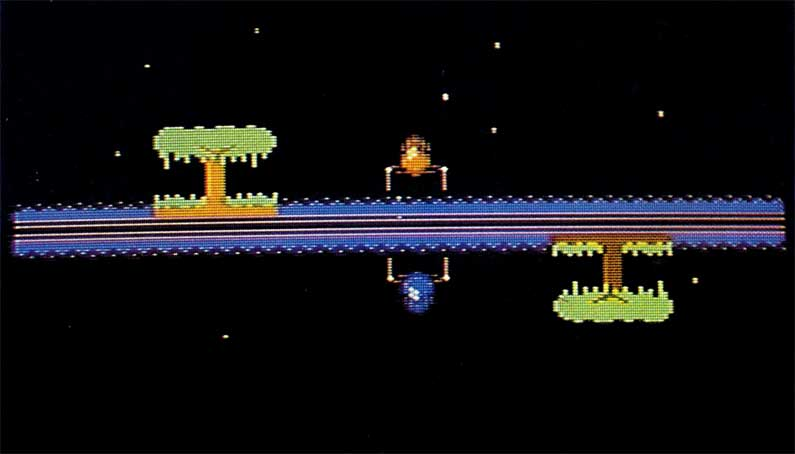
\includegraphics[width=10cm]{src/diary/zzap13_pic1.jpg}%
\caption{An early version of the Sheep planet.}
\end{figure}

\subsubsection{15 February 1986}
The design is taking more concrete shape in my head. I am altering the scroll routine to fit in with my new plans and splitting the screen in the middle. Got the contraflow routines going over garbage data just to see if they work. It seems that they do although there seems to be a slight glitch at high forward accelerations that I'll look into later.

\subsubsection{16 February 1986}
Spent the day designing some planet data and graphics, and stuffed it in to see what the routine looks like with some real data. Looked OK but a bit coarse going at 2 pixels/frametime minimum increment, so I rewrote the stars and planet scroll so that the minimum increment is 1 pixel per frame time. It looks a lot better like that. The planet graphics I did are too coarse, though... I don't really like the way they look, so I may well do a new set tomorrow. The current set is based around a block of data 2 chars x 2 chars, and doesn't look that great.

Did write this really neat routine, though. A complete set of planet graphics takes up 512 bytes of character set data, so I just store the definitions for the top planet and let the computer generate the inverted/reflected set for the bottom planet. Works fine after a little hassle — reflecting multicolour data is a little awkward — but saves storing all those inverted definitions.

\subsubsection{17 February 1986}
Redid the graphics completely, came up with some really nice looking metallic planet structures that I'll probably stick with. Started to write the GenPlan routine that'll generate random planets at will. Good to have a C64 that can generate planets in its spare time. Wrote pulsation routines for the colours; looks well good with some of the planet structures. The metallic look seems to be 'in' at the moment so this first planet will go down well. There will be five planet surface types in all, I reckon, probably do one with grass and sea a bit like 'Sheep in Space', cos I did like that one. It'll be nice to have completely different planet surfaces in top and bottom of the screen. The neat thing is that all the surfaces have the same basic structures, all I do is fit different graphics around each one. Got to sort out the scroll limits tomorrow... at the moment you can shoot right off the end of the planet into garbage data which ain't too cool. Down the clocktower in the evening, cheap beer, 50p a pint, Courage Best promotion. Well good.

\subsubsection{18 February 1986}
Fixed scroll limits and did a little more work on the planet generator routine. Scroll looks really neat, especially at high speed. Very pleasing. Must think about doing the ship controls now.

\subsubsection{19 February 1986}
Wrote the code to put Our Hero (tentatively called B-D) (after the little Indian cigarettes I like) on the planet surface, in the right place, and the right colour, and the right size. Wrote the animation routines that'll be used to make him move. Hooked him up to the scroller so that now he walks left and right under joystick command. Started work on Dark Side set for Colourspace.

\subsubsection{20 February 1986}
Put in gravity routines for the robot — he can now run and jump, too. The grav is nice and low, graceful leaps. Robot will have to jump over features on the planet surface.

\begin{figure}[H]
    \centering
      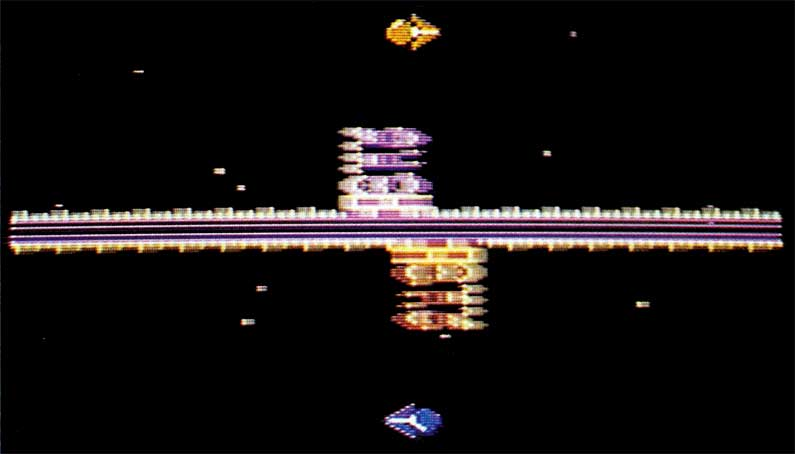
\includegraphics[width=10cm]{src/diary/zzap13_pic2.jpg}%
\caption{An early version of the Mushroom planet.}
\end{figure}

\subsubsection{21 February 1986}
Ship main control mode now complete, with the addition of the 'spaceship' mode: stop the little robot, jump him up and push the stick left and right to make him transform into a spaceship which can really belt over the planet surface. Control feels good, and I'm pleased, cos that's important.

\subsubsection{22-23 February 1986}
Weekend in Cardiff with some mates and Colourspace. Dark Side set finished and demonstrated. Was in a car crash. Left my scarf in Cardiff. Freaked people out on train on way home.

\subsubsection{24 February 1986}
Sprite plex routines written today to reproduce sprites 1-7 on both planets. Works OK. Put in the other 'upside-down' ship controls, work fine but need upside-down sprites defining! At the moment it isn't inverted, uses the same Images as the top one.

\subsubsection{25 February 1986}
Defined the necessary inverted sprites and banged 'em in. They look fine, the mirrored screen and planets scrolling different directions are really bad for the eyes! Tidied up the joystick control to make it less finicky.

\subsubsection{26 February 1986}
Seminar on MSX-2 at Microsoft in Reading. Bit of a booze-up, too smashed to do anything constructive in the afternoon.

\subsubsection{27 February 1986}
Put in planet surface firing for the top ship. The ship lobs out large round bullets while it is on the planet surface — I intend to have certain nasties that can only be properly killed with ground-based fire. The routine works but I am losing every other frame due to interrupt overrun, so I reduce the number of stars on screen to get back about an inch of interrupt time. This does the trick, all cool. Some faffing around with interrupt positioning needed too.

\subsubsection{28 February 1986}
Finished off firing routines of upper ship, added the faster, horizontal fire that the ship produces while flying above the planet surfaces. The whole thing feels nice, good firing response, just the right spacing between the bullets, and a nice transition from ground/airborne firing modes.

\subsubsection{1-2 March 1986}
Bone idle.

\begin{figure}[H]
    \centering
      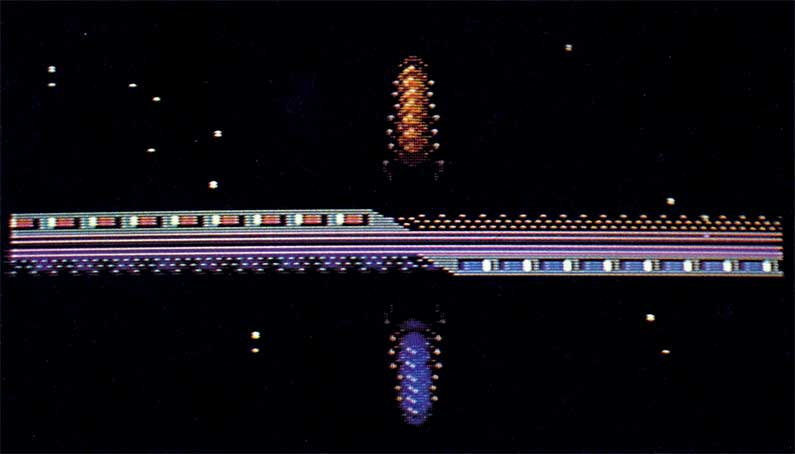
\includegraphics[width=10cm]{src/diary/zzap13_pic3.jpg}%
\caption{An early version of the Mushroom planet.}
\end{figure}

\subsubsection{3 March 1986}
Wrote the extra bullet-handlers to add fire to the lower ship as well as the upper. The lower ship has its own, independent bullets, they can't just be reflections of the upper ship's bullets. The firing is ace. Love it. Especially the gravity on the planet-bound firing, but then I always did go for gravity.

\subsubsection{4-5 March 1986}
Much messing around with graphics for the other planet surfaces, got four defined so far, Metallic, Brick, Country and Mushroom (although I have only half finished the graphics on Mushroom). The afternoon went learning how to set up the new telly I've just bought for doing Colourspace on.

\subsubsection{6 March 1986}
In London, setting up for the ATARI show.

\subsubsection{7-9 March 1986}
Also in London, getting very knackered doing the Atari show. Continuous lightshows, on the hour, every hour, for three days. Went to Laserium Sat nite, crashed on mate's floor, failed TOTALLY to get any sleep. Wrecked by Sunday.

\subsubsection{10 March 1986}
Drove to Ludlow for the second stage of the ZZAP! Challenge. Played games all day, boozer in the evening, crashed the night on La Penn's floor. Ceremoniously burnt the review of Mama Llama with Penn's own lighter. (Next morning Gary Liddon woke to find himself covered in the ashes —Ed)

\subsubsection{11 March 1986}
Got up, read The Beano went to ZZAP! offices to hassle them for a cup of tea but they ran out of tea bags so had to go to restaurant down the road. Drove back from Ludlow. Lots of sheep near Ludlow, you know. Pretty Welsh ones. Set up 8 foot Colourspace screen in Llab. Had mega session on it.

\subsubsection{12 March 1986}
Getting stuff ready for taking to France. Will take 128. Probably won't have much chance to work on Iridis Alpha until I get there, now. Another session on the big Space rig tonight with some Clocktower regulars.

\subsubsection{Tue 18 March 1986 — in France}
Settled in here now. Found an ace black run today, you can go for a whole side of Genesis down it without stopping, but on the second time down I hit a tree stump protruding through the snow, and did an un intentional flying-Yak bit, and landed on a part of my anatomy I'd rather not have landed on. Fired up the 128, finished the Mushroom planet and designed one more, then did a nice fade between planets routine.

\subsubsection{Wed 19 March 1986}
Cloudy weather — makes skiing hard coz you can't see the bumps. Wrote sonix driver and started to phase in some of the FX for walking, jumping etc.

\subsubsection{Thur 20 March 1986}
Still cloudy. Some snow. Had to buy crappy, French headphones to replace my excellent Sony pair that I knackered when I got them tangled up in a chairlift, dammit! Extended the sonix driver and did a few more FX. Sonix take ages, lots of messing around to do before you get it just right.

\subsubsection{Fri 21 March 1986}
Piste all day, back for more SFX, had to rearrange the interrupt sequence to get it all to fit in the frametime.

\subsubsection{Sat 22 March 1986}
Excellent day — bright sun, good snow, didn't start work till late coz I went on skiing so long. Wrote module to link 8 sprites reserved for 'enemy ships' to planetary motion, and also give them each independent velocities. Did a little work on the Pause mode when I got back from the bar.

\subsubsection{Sun 23 March 1986}
Really bad weather, horrible snow that's nearer rain and so sticky you need to be standing on a near-vertical incline before you even start moving. Hit the bar early, then back for mega Guardian session, then a little more work on the pause mode.

\subsubsection{Mon 24 March 1986}
REALLY crappy weather. Got soaked skiing, thawed out in the bar. Retired to room to think about the alien control system while listening to 'The Wall'. Planned it out on paper ready to code later. Got a neat idea for Phase II of the game, thinking along the lines of Batalyx Subgame 1 crossed with a sort of overhead view vertically-scrolling Marble Madness track. Finished off the Pause mode after evening bar. (This'll be the only Pause mode that's been written TOTALLY under the influence of very expensive Guinness).

\begin{figure}[H]
    \centering
      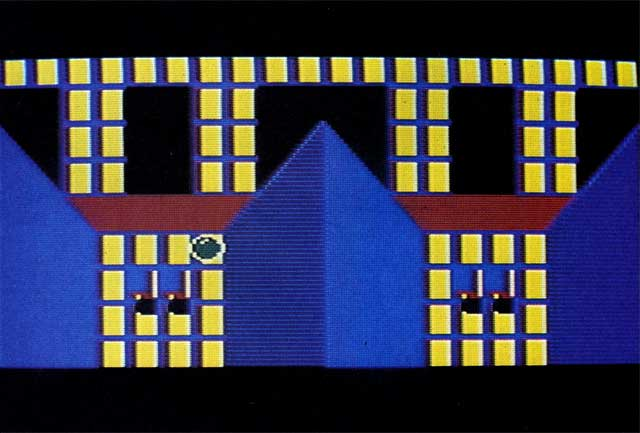
\includegraphics[width=10cm]{src/diary/zzap15_pic1.jpg}%
\caption{An early version of the Bonus Phase.}
\end{figure}

\subsubsection{Tue 25 March 1986}
New snow, much better skiing all round. Linked completed Pause mode to rest of game. Started on alien control system. Went down bar and got absolutely smashed and had amazing discussion on Life, the Universe and Everything. Listened to 'Wish You Were Here' at half-3, in the morning... ace!

\subsubsection{Wed 26 March 1986}
Skiing OK, came back after full day's pistebashing to do some AC System hacking. Hit a terrible awful bug, ran through the code a million times but not got it yet, so down bar to drown sorrows in copious amounts of Guinness.

\subsubsection{Thu 27 March 1986}
Skiing all day then back for the last day's coding in France, I go home tomorrow. Wrestled with the same bug for three hours, was despairing, then noticed a single missing comma in a massive data table that the assembler had neglected, in its infinite wisdom, to flag as an error during assembly, choosing instead to trash the whole data table. Inserted comma; end of bug. Guinness.

\subsubsection{Fri 28/Sat 29 March 1986}
Trains, trains, trains and Frenchmen, ferry, more train, London, underground, train, bus, Tadley, tea, crash.

\subsubsection{Sun 30/Mon 31 March}
Lazy. Didn't do anything, couldn't because me 128 is in France and I need to buy another one, and it's Easter holidays.

\subsubsection{Tue 1 April 1986}
Went into Reading to get a 128D, got it, intended to return and dutifully do some work, but instead met some of the Incentive mob, went to pub (fatal mistake for programmers), all ended back in Tadley for mega-Colourspace session, so fat chance of getting any work done there...

\subsubsection{Wed 2 April 1986}
Set up new 128D, machine is fine but has a noisy fan and sounds like a small but enthusiastic Hoover. Did a little more work on the ACM, not much mind you.

\subsubsection{Thu 3 April 1986}
Went up to London to see Ariola mob and copped some Amiga stuff off them — EA stuff but not Marble Madness yet — they seem quite keen on Iridis Alpha, especially my ideas for phase 2.

\begin{figure}[H]
    \centering
      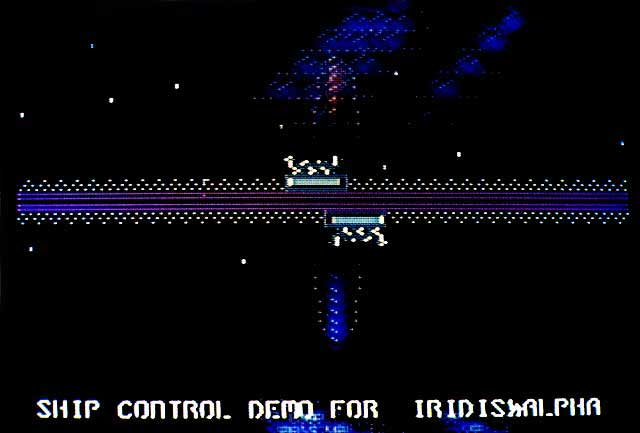
\includegraphics[width=10cm]{src/diary/zzap15_pic2.jpg}%
\caption{Screenshot of Demo Ship Control.}
\end{figure}

\subsubsection{Fri 4 April 1986}
Decided for a break to do a little work on Phase 2 and give Phase 1 a rest. Started at 11 am, finished at 7 am next morning, with a LOT of work done.

\subsubsection{Sat 5 April 1986}
Lots more work done today, I now have a tidy little demo of Phase 2, including complete control system and scrolling background in four different colourschemes, and all inertia routines working. Not bad for a couple days' hacking — got to bed early tonite, 6am!

\subsubsection{Sun 6 April 1986}
Started to get a little sidetracked now, coz I have to get my newsletter done before I go to Lanzarote on Thursday. HAD A MEGA COLOURSPACE SESSION that finished about half-3 then up writing newsletter till 6. One day maybe I get some sleep.

\subsubsection{Mon 7 April 1986}
Did a little more tweaking to phase 2, removing the odd bug I'd found. Then finished newsletter overnight.

\subsubsection{Tue 8 April 1986}
All day working on lightshow for performance at Clocktower this evening. Went good. Got big cheer for 'Stairway to Heaven', and free beer all night.

\subsubsection{Wed 9 April 1986}
Preparing to go away tomorrow. It's a hard life having to keep trekking around to the snow and the beaches, you never seem to get a decent stretch of work done... (hehehe)

\subsubsection{Thu 10/Thu 17 April 1986}
Sun, sea, sand and CAMELS.

\subsubsection{Fri 18 April 1986}
Prepared demos to send off to ZZAP! Couldn't get much serious done because I have to cart all my gear up to London tomorrow for CES Show at Olympia, goes on till Thursday! Then, thank goodness, I get a clear run till the Commodore show, I will at last be able to settle down to some decent coding. Holidays and shows are fine but tend to disrupt you something chronic!!!


\subsubsection{Too Much}
I've decided to drop the individual daily notes for this particular section. I looked at it and there was just too much stuff that was the same on consecutive days, y'know, stuff like May 3: Worked on ACONT. May 4: More work on ACONT. May 5: did stuff for ACONT, etc... etc... What I'll do is try and tell you exactly what's been developed within the game and why it's there.

\subsubsection{ACONT}
This is the bit that I knew would take me ages to write and get glitch free, and the bit that is absolutely necessary to the functioning of the game. The module ACONT is essentially an interpreter for my own 'wave language', allowing me to describe, exactly, an attack wave in about 50 bytes of data. The waves for the first part of IRIDIS are in good rollicking shoot-'em-up style, and there have to be plenty of them. There are five planets and each planet is to have twenty levels associated with it. It's impractical to write separate bits of code for each wave; even with 64K you can run outta memory pretty fast that way, and it's not really necessary coz a lot of stuff would be duplicated. Hence ACONT.

You pass the interpreter data, that describes exactly stuff like: what each alien looks like, how many frames of animation it uses, speed of that animation, colour, velocities in X— and Y— directions, accelerations in X and Y, whether the alien should 'home in' on a target, and if so, what to home in on; whether an alien is subject to gravity, and if so, how strong is the gravity; what the alien should do if it hits top of screen, the ground, one of your bullets, or you; whether the alien can fire bullets, and if so, how frequently, and what types; how many points you get if you shoot it, and how much damage it does if it hits you; and a whole bunch more stuff like that. As you can imagine it was a fairly heavy routine to write and get debugged, but that's done now; took me about three weeks in all I'd say.

\subsubsection{GENESYS}
With ACONT running I had to implement the GENESYS routine, which actually oversees passing data to ACONT, finding out what aliens to unleash depending on what wave we're on and what planet, arranging for shot aliens to be cleaned up and new ones sent out to replace them. I had ACONT running with a limited, one-wave only version of GENESYS at the Commodore show, where a demo of IRIDIS was running non-stop on our stand. I stayed up till three, the morning of the show, preparing a neato title screen with one of my sprite starfields, the game's title and an animated demo, but hardly anyone saw the demo anyway coz they were all playing the game.

I was surprised at the response, after all the thing was only a demo, the scoring was erratic, there was only one wave and you couldn't get killed, but still it was heavily played at the show. People seemed to get into it, enjoying the raw blasting of the thing. One lad even begged to buy my development demo off me, he was just getting off on the blasting and wanted to carry on at home!

\begin{figure}[H]
    \centering
      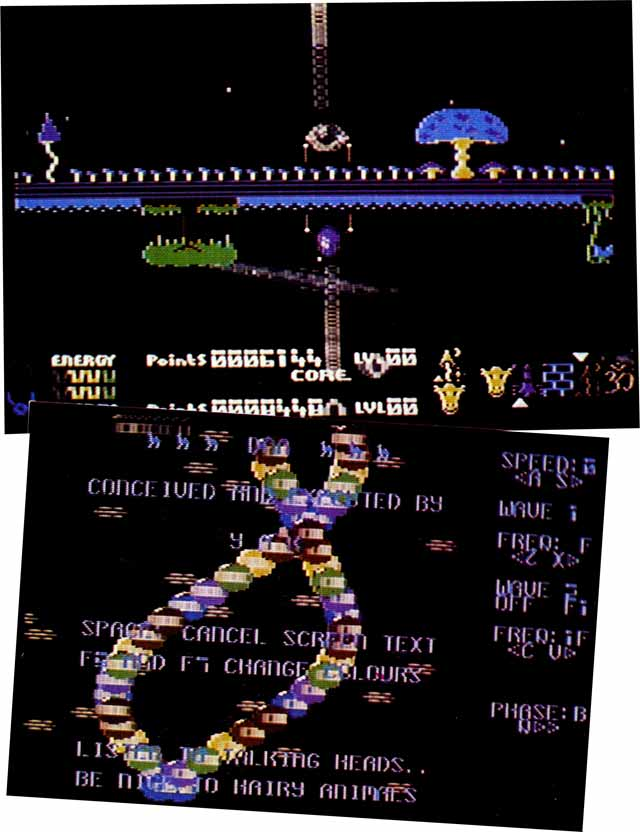
\includegraphics[width=10cm]{src/diary/zzap16_pic1.jpg}%
\caption{An early version of the Mushroom planet and the DNA demo.}
\end{figure}

\subsubsection{CBM}
The Commodore show was fun, as ever: I met a lot of good people there, and did some serious partying... I don't think Mat or Psy or Wulf are going to forget THAT night for a while. Everything they say about programmers is TRUE. Make of that what you will.

\subsubsection{Fatigue}
After CBM was over, I spruced up GENESYS and got it to the point where I could actually start doing the attack waves. That's more or less what I've been doing up till now: designing sprite sequences, flight paths, puzzles in some levels, testing 'em to make sure they are not too difficult for mere mortals. After doing about 40 waves and realising that there's still another 60 to go, 'Attack Wave Fatigue' starts to show up, but you just gotta plug on and get 'em done. At the time of writing this I've done 66 of them. I also did a lot of tweaking to the flight mechanics, and designed the display panel and got its various gauges and meters running.

\subsubsection{The Core}
IRIDIS is unusual in offering two scores, one for each ship. Each ship also has an individual energy bank. As you collide with stuff, you lose energy, naturally. If you lose it all, you DIE. So you shoot some stuff, and as you kill, so energy gets added to your ship's bank. You gotta watch it, though, coz if you collect up too MUCH energy, guess what happens? Yup — you DIE.

Thus, gameplay on IRIDIS involves frequent deliberate collisions, as well as shooting, in order to keep the energy balance cool. There is another way, too: fill up both ships with energy, and then land on the platform (which in the game is known as the CORE). The CORE accepts your excess energy, leaving you with comfortably half-full tanks. Also, if you're copping really heavy flak from a particularly vindictive attack sequence, you can nip along to the CORE and reclaim any energy you might have stashed there during easier times. (Author's note: this new Sabbath album is AWESOME).

Filling up the CORE entirely will grant you a bonus and allow access to Phase II of IRIDIS, that vertically-scrolling thing I mentioned in the last set of notes. You'll have to run the gauntlet of the scrolling course and dump your energy at the end for a mega bonus, then return to main IRIDIS and continue climbing the levels.

Once I finish the attack waves, I gotta tie up all of Phase One before going in to finish Phase II. A rather mean thing is going to be the scoring system — the faster you fly, the more points you get for each killing. Standing still and blasting will earn you no points at all. Flying about at mach III like an F-111 pilot over Libya will net the most points.

\subsubsection{Distractions}
IRIDIS ALPHA being brought to you despite the following distractions:

Ronnie James Dio in concert (twice)
Colourspace II starting to get written on the ST
THRUST
Time Bandit, Star Raider, Spy Hunter, Joust on the ST
The Incredible Bioxwich Trip (Too Weird for Words)
Invisible Touch
Blade Runner
DNA (GOTO YAK and DOWNLOAD!)
My assembler politely informing me that every single branch in the whole bit of code was out of range, then trashing my disk
Compunet and all the heroes thereon

\subsubsection{I'm a Hero...}
As I write this, IRIDIS is nearly completed. I just gave the first pre-production prototype to one of the Hewson mob, ready to be duplicated and dished out to the press at the press launch on Thursday. Getting it ready for the press launch has meant a couple of all-nighters over the last weekend, but it's worth it — I got it done, so I'm a hero...

\subsubsection{Phase II}
Basically, since last time I wrote, I've been doing Phase II most of the time. I finished off the tricky ACONT routine, and defined the data for all 100 attack waves, then I got down to doing Phase II which was interesting, 'coz it's a vertically scrolling game, and I don't usually do vert-scrollers.

Although I described it before as a loose cross between Phase I of BATALYX and MARBLE MADNESS, it is actually closer to a cross between Phase I of BATALYX and pinball. When you're playing it, you get the odd feeling of actually being the pinball as poor Gilby ricochets off everything in sight at high Delta V. I once saw a pinball game being sold in America which claimed that 'you are the pinball', but when I played it, it turned out to be just a scrolling pin-table, and you were the flippers, not the ball. In Phase II of IRIDIS you are definitely the ball. No doubt about it. And you get hotly pursued by four flying eyeballs.

\begin{figure}[H]
    \centering
      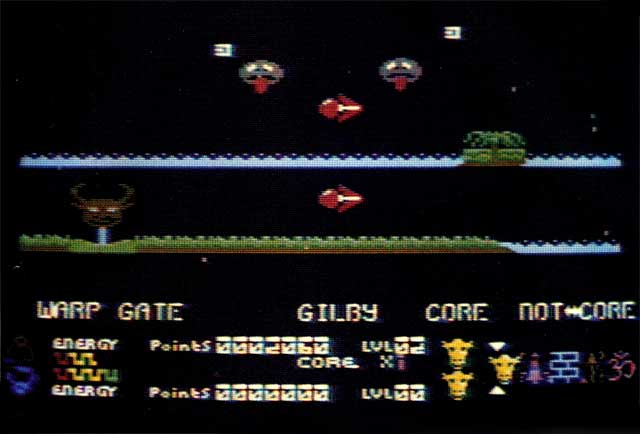
\includegraphics[width=10cm]{src/diary/zzap17_pic1.jpg}%
\caption{
A mutated Gilby is surrounded by enemy vessels.
}
\end{figure}

In Phase II there are 256 possible courses, each one different - I worked this trick by generating each level randomly out of 20 or 30 basic components. But, to ensure that each level would be consistent from game to game, I seeded the random number generator with the level number each time the course gets generated. You get distinct courses for each level, but Level 1 will always look like Level 1, for example, and won't be random every time you go in, so, you can make maps and learn the courses as you play. It's neat, 'coz it looks as if I carefully designed and stored all those different courses, and all I really did was call the ol' RAN\$ routine a couple of times. I love cheating.

\subsubsection{Well 'ard}
I've included a neat high score table, and a new system of graphically displaying the player's progress through the game, as well as progressive opening of the Warp Gate as the player's skill increases. The game now starts up with only one planet, so that new players have a chance without it all being too complicated. Once the third wave (Licker Ships — well 'ard) is passed, the second planet becomes available. As the player goes through the game, more planets become available, and he can sustain his game by earning extra lives on Phase II.

I had a bit of room knocking about under the Kernal so I fitted in my DNA demo; it's available from inside MIF (the little pause mode sub-game I wrote in France).

There's also a title page under there, and a twenty-name Hi Score table (full of default entries like YAK, PSY and MAT, RATT, and various other Compunetters)...

All that's really left for me to do now is final debug, tidying up of rough edges, and add a couple of surprises... maybe. I have a week or so to do that, then it's the end-of-July deadline and if I don't make it I get parts of my anatomy chopped off. I'll do it. I'm a hero, like I said, without even playing BIGGLES.

\begin{figure}[H]
    \centering
      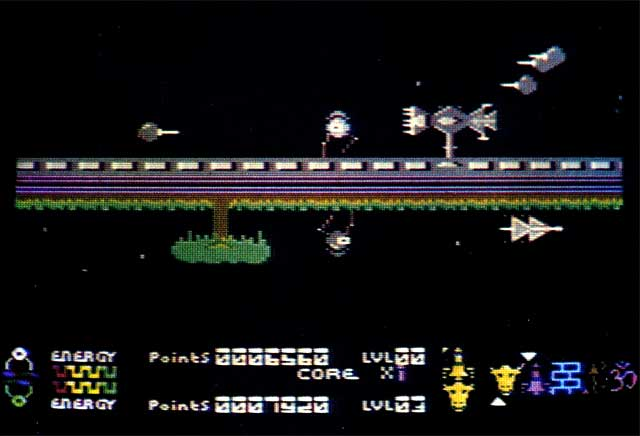
\includegraphics[width=10cm]{src/diary/zzap17_pic2.jpg}%
\caption{
The cute 'n' cuddly Gilbies walk along the surfaces of the duo planets
}
\end{figure}

\subsubsection{A good 'un}
One thing I like about IRIDIS is that it's got very playable, more so than just about any other of my games.

I realised this when I passed the point that comes whenever you write a game: there's always a day when the game stops being just a collection of scroll routines and stuff that you have to run and debug, and starts to become a real game. You know it's happened because you find yourself testing the game even when it doesn't need any testing, and suddenly all your mates know the SYS number to get it started, and use it frequently. IRIDIS passed that point a while back, and it's now well into the 'lights out, heavy rock music on, colour on monitor nice 'n' high, let's go give 'em HELL!' stage. It's great when you've done the high score table and you can rack up a good 'un, too. Remember way back when I started and had nothing much beyond a star scroll, and I said that IRIDIS was gonna blast like crazy? I was right... hehe.

\subsubsection{I'm off}
After I've finished, I'm off to Corfu for a couple of weeks well-earned rest doing nothing but parascending, lying on the beach, and getting paralytic at Mrs Platypus's bar.

And playing SATAN OF SATURN, the local video game. And listening to 'Brothers in Arms'.

Finally, then, I will leave you, having chronicled the progress of IRIDIS from conception to birth. If you love a blaster then I think you'll like IRIDIS. It's been heavy work, but ultimately worth it, I think.

Long live Gilby! Death to the Zzyaxians!

\subsubsection{Distractions}
IRIDIS ALPHA being brought to you by YAK the hairy, with the support of the Coca Cola Company, Atari UK, Pink Floyd and Genesis, Heavy Metal, Wadworths 6X, Ratt, Ben, Mat, Psy, Wulf, etc, Compunet, Dried leaves diffused in boiling water, MIND WALKER, MARBLE MADNESS, STAR GATE, Taun-Tauns, Camels, Llamas, Sheep and Goats... MARBLE MADNESS...

Assembled on a C128 using a partially-finished JCL assembler and the horrible, slow Commodore disk drives. Next time I'm gonna use a 6502 X-ASM running in 2.5 Megabytes of RAM on me trusty ST...

Sourced from https://codetapper.com/c64/diary-of-a-game/iridis-alpha/
